%%%%%%%%%%%%%%%%%%%%%%%%%%%%%%%%%%%%%%%%
%%%%%  xPhO LaTeX Beamer Template  %%%%%
%%%%%  Date: 17/03/2025            %%%%%
%%%%%  Authors:                    %%%%%
%%%%%       Nguyen Thanh Long      %%%%%
%%%%%       Nguyen Le Mai Huong    %%%%%
%%%%%       Nguyen Minh Phuong     %%%%%
%%%%%%%%%%%%%%%%%%%%%%%%%%%%%%%%%%%%%%%%

\documentclass[aspectratio=169, t]{beamer} % Ratio 16:9
\usepackage[T5]{fontenc}
\usepackage{lmodern}
\usepackage{graphicx} 
\usepackage{array}
\usepackage{longtable} % for long table

\usepackage{amsmath}

\usepackage{chngcntr}
\counterwithin{figure}{section}

\renewcommand{\familydefault}{\sfdefault} % Font

\usepackage{caption}
\usepackage{siunitx}

% \definecolor{BlueDefault}{rgb}{0.2,0.2,0.7}
\definecolor{BlueDefault}{RGB}{14,47,95}


% Hide navigation 
\setbeamertemplate{navigation symbols}{}

% Setup background
\newcommand{\normalbackground}{%
    \usebackgroundtemplate{
\includegraphics[width=\paperwidth,height=\paperheight]{Background/Normal_slide_xPhO.pdf}}%
}

\newcommand{\titlebackground}{%
    \usebackgroundtemplate{
\includegraphics[width=\paperwidth,height=\paperheight]{Background/Title_slide_xPhO.pdf}}%
}

% Change the title color to white
\setbeamercolor{frametitle}{fg=white} 

% push the title up by \raisebox
\setbeamertemplate{frametitle}{%
    \vspace{0.3em}
    \hspace{-1em} \insertframetitle
    % \vspace{2mm}
}

% Number of slide
\setbeamertemplate{footline}{%
    \hfill
    \insertframenumber/\inserttotalframenumber
    \hspace{7.5mm}
    \vspace{3.5mm}
}

%% Make Table of Contents %%
\AtBeginSection[]{
  \begin{frame}
  \frametitle{Mục lục}
  \tableofcontents[currentsection]
  \end{frame}
}

%% Section numbering %%
\setbeamertemplate{section in toc}[sections numbered]
\setbeamertemplate{subsection in toc}[subsections numbered]


\renewcommand{\figurename}{Hình}
\renewcommand{\tablename}{Bảng}


%%%%% Bibliography %%%%%
\usepackage[backend=biber,style=ieee]{biblatex}
\addbibresource{citation.bib}

\usepackage{url}
\usepackage{hyperref}
\hypersetup{
	colorlinks=true,
	linkcolor=BlueDefault,
	filecolor=BlueDefault,
    citecolor=BlueDefault,
	urlcolor=BlueDefault,
	pdftitle={Overleaf Example},
	pdfpagemode=FullScreen,
}

\begin{document}

\titlebackground

\begin{frame}[noframenumbering]
    \thispagestyle{empty}
    \bfseries
    \begin{flushleft}
        \vfill
        \vspace{5mm}
        \textcolor{BlueDefault}{\huge \bfseries MA TRẬN TRONG CƠ HỌC \vspace{2mm} \\ VÀ MÔ PHỎNG CÁNH TAY ROBOT} \\
        \vspace{10mm}
        \textcolor{black}{\large \bfseries Người trình bày: Nguyễn Thành Long}
        \vfill
    \end{flushleft}
\end{frame}

\normalbackground

\section{Giới thiệu chung về ma trận và động học}

\subsection{Vector, tọa độ suy rộng và ví dụ robot Scara}

\begin{frame}{Robot Scara 4 bậc tự do}
    \begin{columns}
        \column{0.5\textwidth}
        \begin{itemize}
            \item Robot Scara có 4 bậc tự do biểu diễn qua các tọa độ: \( q = [q_1, q_2, q_3, q_4]^T \).
            \item 3 khớp quay: \(q_1\), \(q_2\), \(q_4\).
            \item 1 khớp tịnh tiến: \(q_3\).
        \end{itemize}
        \begin{figure}
            \centering
            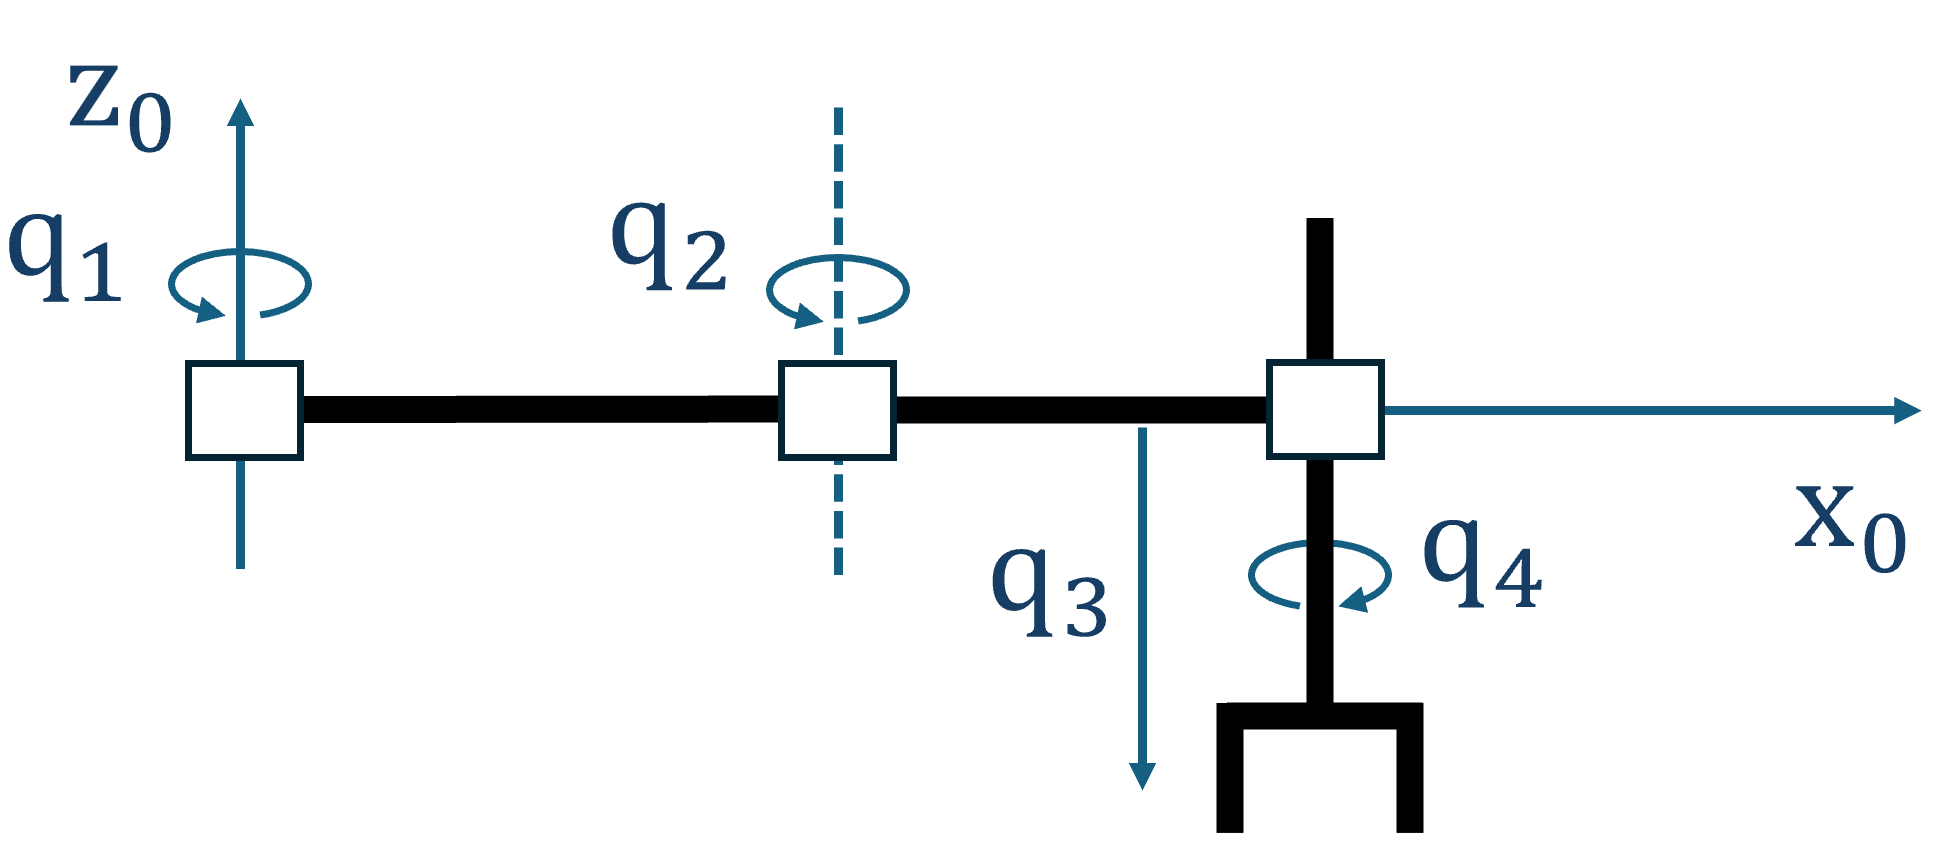
\includegraphics[width=0.8\linewidth]{Figures/Scara_xOz.png}
            \caption{Mặt cắt phương xOz của Robot Scara.}
            \label{fig:Scara_xOz}
        \end{figure}
        \column{0.5\textwidth}
        \begin{figure}
            \centering
            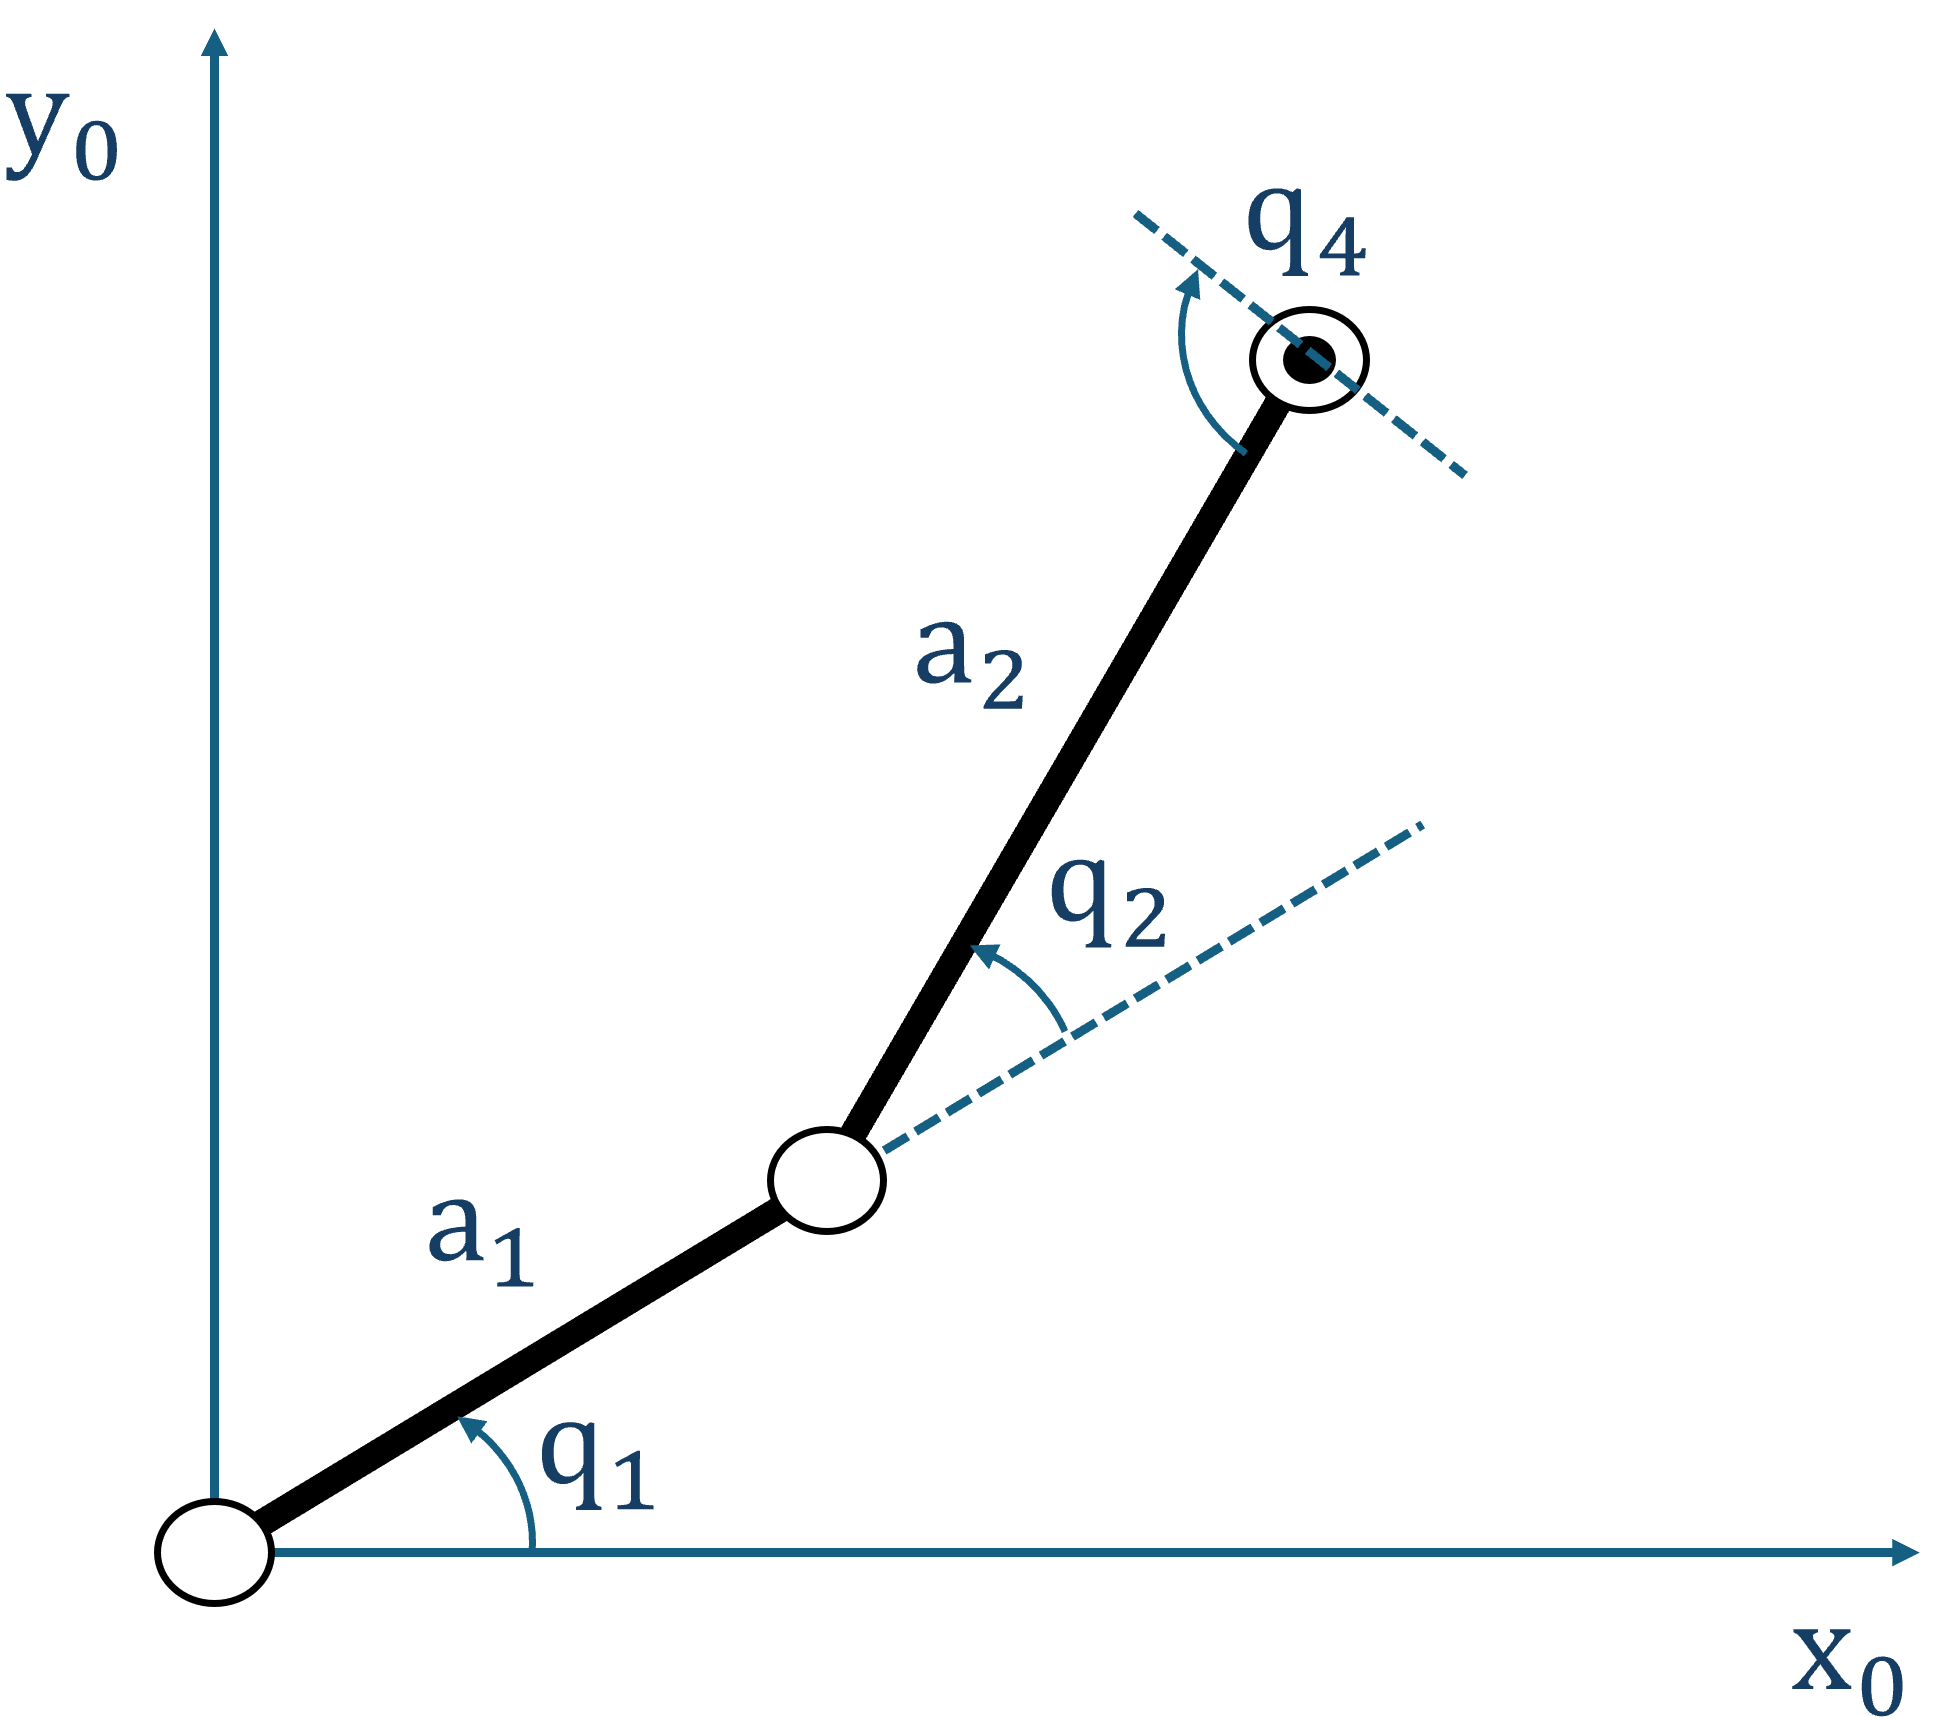
\includegraphics[width=0.8\linewidth]{Figures/Scara_xOy.png}
            \caption{Mặt cắt phương xOy của Robot Scara.}
            \label{fig:Scara_xOy}
        \end{figure}
    \end{columns}
\end{frame}

\begin{frame}{Phép toán cơ bản với ma trận}
    \begin{itemize}
        \item Nhân một số với một ma trận.
    \end{itemize}
    {\footnotesize
    \begin{equation}
        P =
        a_1
        \left[ \begin{array}{c}
            \cos \left( q_1 \right) \\
            \sin \left( q_1 \right) \\
            0
        \end{array} \right]
        +
        a_2
        \left[ \begin{array}{c}
            \cos \left( q_1 + q_2 \right) \\
            \sin \left( q_1 + q_2 \right) \\
            0
        \end{array} \right]
        +
        q_3
        \left[ \begin{array}{c}
            0 \\
            0 \\
            -1
        \end{array} \right]
        =
        \left[ \begin{array}{c}
            a_1 \cos \left( q_1 \right) + a_2 \cos \left( q_1 + q_2 \right) \\
            a_1 \sin \left( q_1 \right) + a_2 \sin \left( q_1 + q_2 \right) \\
            -q_3
        \end{array} \right].
    \end{equation}
    }
    
    \begin{itemize}
        \item Nhân một ma trận với một ma trận.
    \end{itemize}
    {\footnotesize
    \begin{equation}
        \left[ \begin{array}{ccc}
            1 & 2 & 3 \\
            4 & 5 & 6
        \end{array} \right]
        \times
        \left[ \begin{array}{cc}
            7 & 8 \\
            9 & 10 \\
            11 & 12
        \end{array} \right]
        =
        \left[ \begin{array}{cc}
            1 \cdot 7 + 2 \cdot 9 + 3 \cdot 11 & 1 \cdot 8 + 2 \cdot 10 + 3 \cdot 12 \\
            4 \cdot 7 + 5 \cdot 9 + 6 \cdot 11 & 4 \cdot 8 + 5 \cdot 10 + 6 \cdot 12
        \end{array} \right]
        =
        \left[ \begin{array}{cc}
            58 & 64 \\
            139 & 154
        \end{array} \right].
    \end{equation}  
    }
    \begin{itemize}
        \item Ma trận chuyển vị
    \end{itemize}
    \begin{equation}
        \left[ \begin{array}{ccc}
            1 & 2 & 3 \\
            4 & 5 & 6
        \end{array} \right]^T
        =
        \left[ \begin{array}{cc}
            1 & 4 \\
            2 & 5 \\
            3 & 6
        \end{array} \right].
    \end{equation}
\end{frame}

\begin{frame}{Ma trận Jacobian và liên hệ vận tốc giữa các tọa độ}
    \begin{columns}
        \column{0.5\textwidth}
            \begin{itemize}
                \item Cho hai hệ tọa độ: \( q = \left[ q_1, q_2, q_3 \right]^T\) và \( P = \left[ x, y, z \right]^T\).
                \item Dựa vào phép đạo hàm toàn phần
            \end{itemize}
            \begin{align}
                \dot{x} &= \dfrac{\partial x}{\partial q_1} \dot{q}_1 + \dfrac{\partial x}{\partial q_2} \dot{q}_2 + \dfrac{\partial x}{\partial q_3} \dot{q}_3, \\
                \dot{y} &= \dfrac{\partial y}{\partial q_1} \dot{q}_1 + \dfrac{\partial y}{\partial q_2} \dot{q}_2 + \dfrac{\partial y}{\partial q_3} \dot{q}_3, \\
                \dot{x} &= \dfrac{\partial x}{\partial q_1} \dot{q}_1 + \dfrac{\partial z}{\partial q_2} \dot{z}_2 + \dfrac{\partial z}{\partial q_3} \dot{q}_3.
            \end{align}
        \column{0.5\textwidth}
            \begin{itemize}
                \item Ma trận Jacobian
            \end{itemize}
            \begin{equation}
                J = \left[ \begin{array}{ccc}
                    \dfrac{\partial x}{\partial q_1} & \dfrac{\partial x}{\partial q_2} & \dfrac{\partial x}{\partial q_3} \\
                    \dfrac{\partial y}{\partial q_1} & \dfrac{\partial y}{\partial q_2} & \dfrac{\partial y}{\partial q_3} \\
                    \dfrac{\partial x}{\partial q_1} & \dfrac{\partial z}{\partial q_2} & \dfrac{\partial z}{\partial q_3}
                \end{array} \right].
            \end{equation}
            \begin{itemize}
                \item Ứng dụng: \(\dot{P} = J \dot{q}\).
            \end{itemize}
    \end{columns}
\end{frame}

\begin{frame}{Ma trận Jacobian và liên hệ vận tốc giữa các tọa độ}
    \begin{itemize}
        \item Ứng dụng cho Robot Scara.
    \end{itemize}
            \begin{align}
                \dot{x} &= \left[ -a_1 \sin \left( q_1 \right) - a_2 \sin \left( q_1 + q_2 \right) \right] \dot{q}_1 - a_2 \sin \left( q_1 + q_2 \right) \dot{q}_2, \\
                \dot{y} &= \left[ a_1 \cos \left( q_1 \right) + a_2 \cos \left( q_1 + q_2 \right) \right] \dot{q}_1 - a_2 \cos \left( q_1 + q_2 \right) \dot{q}_2, \\
                \dot{z} &= -\dot{q}_3.
            \end{align}
    \begin{itemize}
        \item Tính độ lớn vận tốc
    \end{itemize}
    \begin{equation}
        v^2 = \dot{x}^2 + \dot{y}^2 + \dot{z}^2
        = \left[ \begin{array}{ccc}
            \dot{x} & \dot{y} & \dot{z}
        \end{array} \right]
        \left[ \begin{array}{c}
            \dot{x} \\
            \dot{y} \\
            \dot{z}
        \end{array} \right]
        = \dot{P}^T \dot{P}
        = \dot{q}^T \left( J^T J \right) \dot{q}.
    \end{equation}
\end{frame}

\subsection{Phép toán cơ bản với ma trận}

\subsection{Jacobian và liên hệ vận tốc giữa các hệ tọa độ}

\section{Động lực học robot}

\subsection{Động năng và ma trận quán tính}

\begin{frame}{Động năng và ma trận quán tính}
    \begin{itemize}
        \item Động năng:
    \end{itemize}
    \begin{equation}
        T = \sum_{i=1}^N \dfrac{1}{2} v_i^T m_i v_i + \sum_{j=1}^M \dfrac{1}{2} \omega_j I_j \omega = \dfrac{1}{2} \dot{q}^T \left( \sum_{k=1}^L J_k^T m_k J_k \right) \dot{q} = \dfrac{1}{2} \dot{q}^T H \dot{q}.
    \end{equation}
    \begin{itemize}
        \item Ma trận quán tính
    \end{itemize}
    \begin{equation}
        H = \sum_{k=1}^L J_k^T m_k J_k.
    \end{equation}
\end{frame}

\subsection{Phương trình động lực học đầy đủ và ma trận Christoffel}

\begin{frame}{Phương trình động lực học và ma trận Christoffel}
    \begin{columns}
        \column{0.4\textwidth}
        \begin{itemize}
            \item Hàm Lagrangian: \( L = K - U\)
            \item Phương trình Euler Lagrange:
        \end{itemize}
        \begin{equation}
            \dfrac{d}{dt} \left( \dfrac{\partial L}{\partial \dot{q}_i} \right) - \dfrac{\partial L}{\partial q_i} = 0.
        \end{equation}
        Phân tách hàm Lagrangian và bổ sung lực suy rộng
        \begin{equation}
            \dfrac{d}{dt} \left( \dfrac{\partial T}{\partial \dot{q}_i} \right) - \dfrac{\partial T}{\partial q_i} = - \dfrac{\partial U}{\partial q_i} + F_i.
        \end{equation}
        \column{0.6\textwidth}
        \begin{itemize}
            \item Lời giải tổng quát
        \end{itemize}
        \begin{equation}
            H(q) \ddot{q} + C(q, \dot{q}) \dot{q} = -\nabla U(q) + F.
        \end{equation}
        \begin{itemize}
            \item Phần tử hàng \(i\) cột \(j\) của ma trận Chrisoffel
        \end{itemize}
        \begin{equation}
            C_{ij} = \sum_{k=1}^{n} \frac{1}{2} \left( \frac{\partial H_{ik}}{\partial q_j} + \frac{\partial H_{jk}}{\partial q_i} - \frac{\partial H_{ij}}{\partial q_k} \right) \dot{q}_k.
        \end{equation}
    \end{columns}
\end{frame}

\subsection{Mô phỏng chuyển động bằng phương pháp số}

\begin{frame}{Mô phỏng hệ Robotic bằng phương pháp số}
    \begin{itemize}
        \item Hệ phương trình vi phân
    \end{itemize}
    \begin{align}
        \dfrac{d}{dt} q &= \dot{q}, \\
        \dfrac{d}{dt} \dot{q} &= H(q)^{-1} \left[ - C(q,\dot{q}) \dot{q} -\nabla U(q) + F \right].
    \end{align}
    \vspace{-5mm}
    \begin{itemize}
        \item Lấy sai phân, rời rạc hóa biểu thức trong mô phỏng số
    \end{itemize}
    \begin{align}
        q|_{t+\Delta t} &= q|_{t} + \dot{q} \Delta t, \\
        \dot{q}|_{t+\Delta t} &= \dot{q}|_t + H(q)^{-1} \left[ - C(q,\dot{q}) \dot{q} -\nabla U(q) + F \right] \Delta t.
    \end{align}
    \vspace{-5mm}
    \begin{itemize}
        \item Chọn \(\Delta t\) rất nhỏ và tiến hành rất nhiều vòng lặp, thu được đồ thị của \(q\) và \(\dot{q}\) theo thời gian.
    \end{itemize}
\end{frame}

\section{Ma trận còn có thể làm những gì trong cơ học?}

\subsection{Bảng Denavit–Hartenberg}

\input{Slides/Denavit–Hartenberg}

\subsection{Thay thế ma trận Christoffel?}

\begin{frame}{Thay thế ma trận Christoffel?}
    \begin{itemize}
        \item Phương trình động lực học tổng quát sử dụng tích Kronecker \cite{Tuan_Chung_Khoa_Phong_2019}:
    \end{itemize}
    \begin{equation}
        H(q) \ddot{q} + C(q) \dot{q} \otimes \dot{q} = - \nabla U + F.
    \end{equation}
    \begin{itemize}
        \item Ma trận hướng tâm/Coriolis \(C(q)\) được tính bằng biểu thức
    \end{itemize}
    \begin{equation}
        C(q) = \dfrac{\partial H(q)}{\partial q} - \dfrac{1}{2} \left( \dfrac{\partial \text{vec}(H)}{\partial q} \right)^T.
    \end{equation}
\end{frame}

\begin{frame}[allowframebreaks]{Tài liệu tham khảo}
    \printbibliography
\end{frame}

\end{document}